%
\section{Description of HMOG features} \label{sectionFeatures}



We define two types of HMOG features: grasp {\em resistance} and grasp {\em stability}. These features are computed from data collected using three sensors: accelerometer, gyroscope, and magnetometer. Because HMOG features aim to capture the subtle micro-movements and orientation patterns of a user while tapping on the screen, we extract HMOG features from signals collected {\em during} or {\em close to} tap events.  
Computation of grasp stability and resistance features is discussed next.
%




%
%
%
%
%
%


%
%



\subsection{Grasp Resistance Features} 
Grasp resistance features measure the resistance of a hand grasp to the forces (or pressures) exerted by touch/gesture events. We quantify resistance as the change, or perturbation, in movement (using readings from accelerometer), orientation (from gyroscope) and magnetic field (from magnetometer), caused by a tap event. 


\begin{table}[htbp]  \caption{Notation.}\label{notation-1}

  \centering \resizebox{.5\textwidth}{!}{
  \begin{tabular}{@{} |c|l| @{}}
    \hline
Sensor & Accelerometer or Gyroscope or Magnetometer. \\\hline   
 $X$, $Y$, $Z$ & Time series of sensor readings in $x$, $y$, and $z$ axes respectively\\ \hline
 $Z_1, \ldots, Z_n$ & Individual sensor readings in $z$ axis collected at time \\ &$t_1, \ldots, t_n$ respectively \\\hline
    $M$ & Time series of magnitude of sensor reading, where each \\ &element $M_i$ is computed as $\sqrt{(X_i^2+Y_i^2+Z_i^2)}$ \\ \hline
    $t_{start}$ & Start time of a tap event \\ \hline
    $t_{end}$ & End time of a tap event \\ \hline
    $t_{max\_in\_tap}$ & Time between $t_{start}$ and $t_{end}$ at which the reading from a \\&sensor   reaches its highest value \\ \hline
    $t_{min}$ & Time when stability is achieved after the tap event has ended \\ \hline
    $t_{before\_center}$ & Center of the 100 ms window before a tap \\ \hline
    $t_{after\_center}$ & Center of the 100 ms window after a tap \\ \hline
    \texttt{avg100msBefore} & Average of sensor readings in a 100~ms  window before start \\ \texttt{avg100msAfter}&  time and after end time, respectively\\ \hline
    \texttt{avgTap} & Average of readings during tap events \\ \hline
    $t_{min}$ & Time when stability is achieved after the tap event has ended\\
    \hline
  \end{tabular}}
\end{table}


%

We extracted five grasp resistance features from accelerometer, gyroscope, and magnetometer, over four dimensions (magnitude, $x$, $y$, and $z$ axes), leading to $5 \times 3 \times 4 = 60$ features. For simplicity of exposition, we describe grasp resistance features only on the $z$ axis. We also extracted the same features from $X$, $Y$, and $M$. Our notation is summarized in Table~\ref{notation-1}. Figure~\ref{fig:drawingStabilityFeatures} illustrates variables used in features 3 through 5.
\begin{enumerate}
\item Mean of $Z$ during taps. %
\item Standard deviation of $Z$ during taps.
%
%
\item Difference in $Z$  readings before and after a tap event. Let \texttt{avg100msBefore} be the average of $Z$ readings in a 100~ms  window before tap start time, and \texttt{avg100msAfter} be the average of $Z$ readings in a 100~ms  window after tap end time. We calculated this feature as the difference between \texttt{avg100msAfter} and \texttt{avg100msBefore}.
\item Net  change in $Z$ readings caused by a tap. Let  \texttt{avgTap} be the average of $Z$ readings during a tap event. We calculate this feature as  \texttt{avgTap - avg100msBefore}.
\item Maximum change in $Z$ readings caused by a tap. Let \texttt{maxTap} be the maximum $Z$ reading during a tap event. This feature is calculated as 
 \texttt{maxTap - avg100msBefore}.
\end{enumerate}




%
\subsection{Grasp Stability Features} 
Stability features quantify how quickly the perturbations caused by a finger-force from a tap event disappear after the tap event is complete.
%
%
We compute grasp stability features as follows:
(Figure~\ref{fig:drawingStabilityFeatures} illustrates variables used in the features.)
%
%
%
%
%

\begin{figure}[tb]
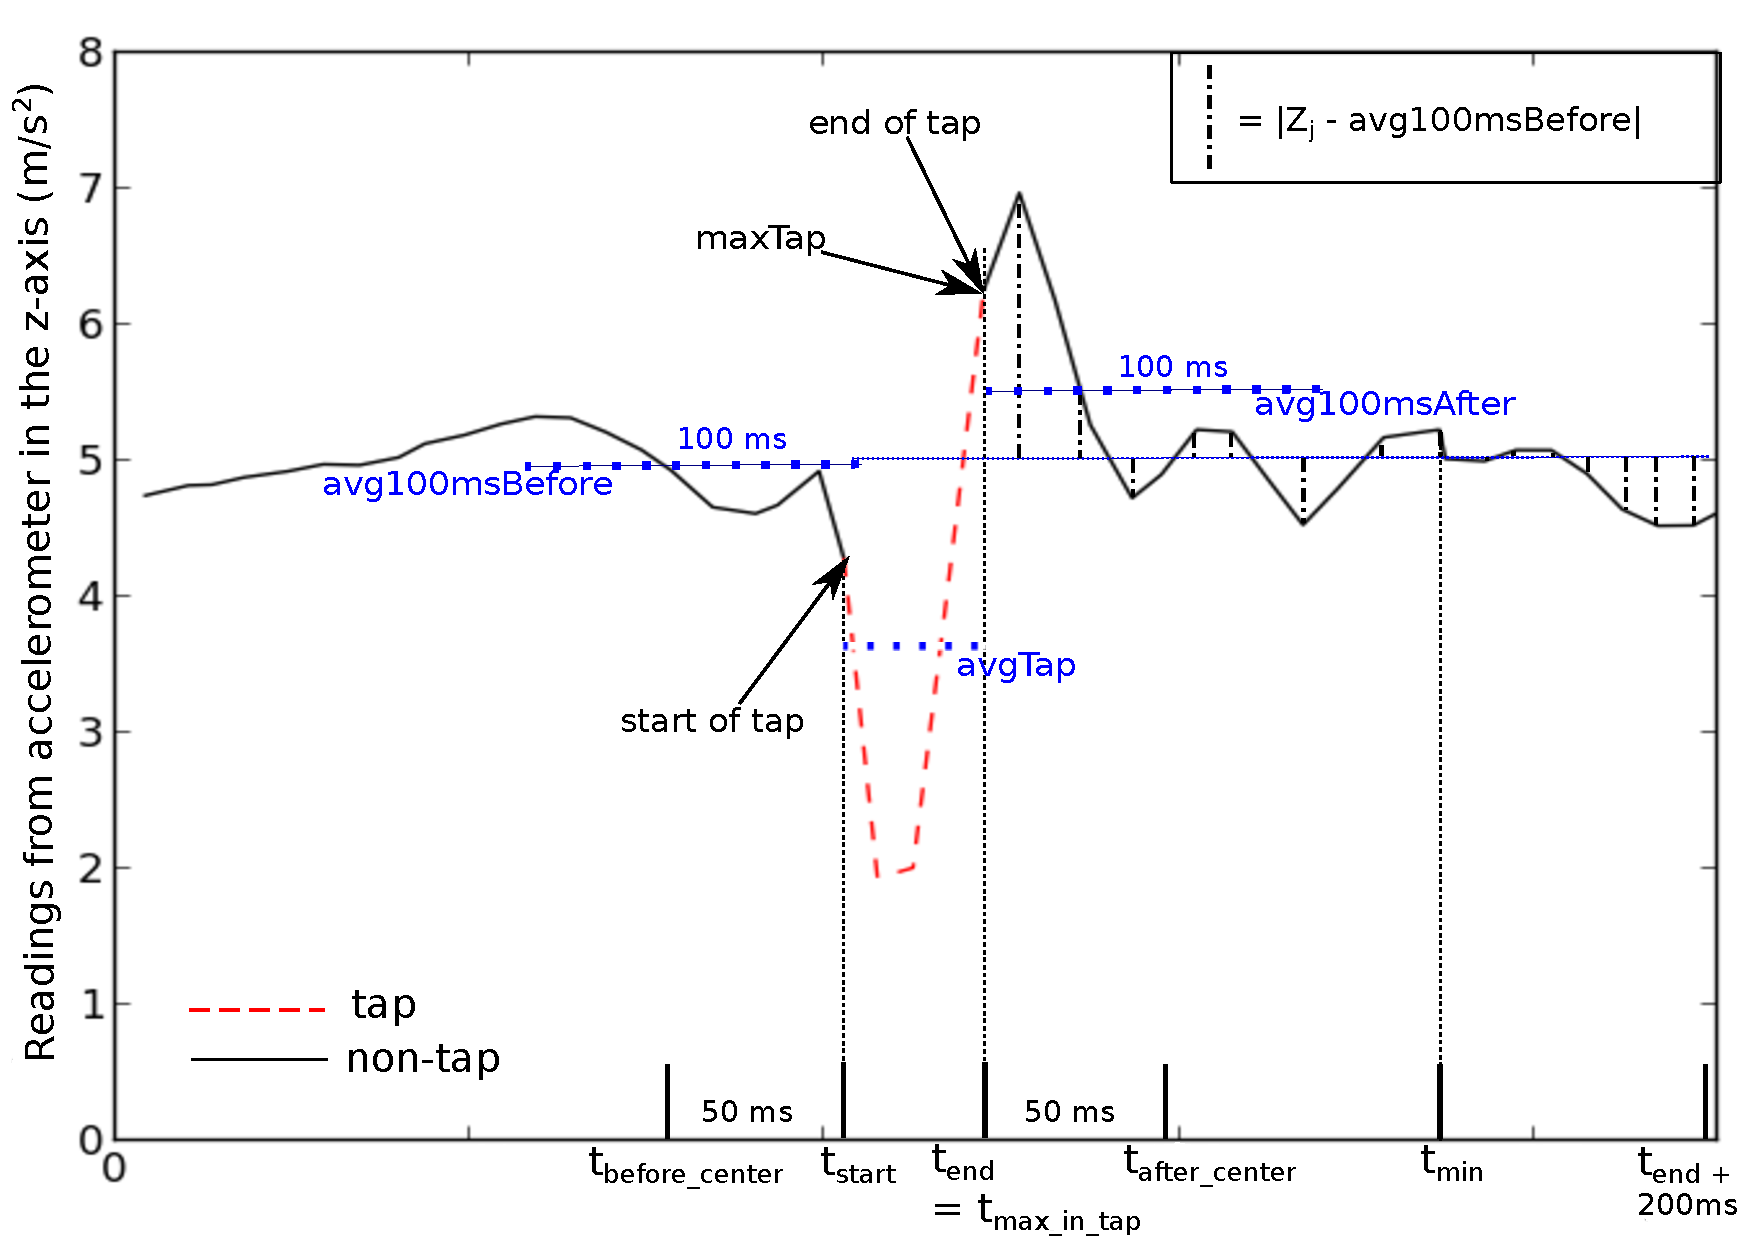
\includegraphics[width=0.96\linewidth]{plots/drawingStabilityFeaturesNewNewSignal.pdf}
\caption[]{Illustration of key variables for computing grasp {\em resistance} features 3-5 and grasp {\em stability} features 1-3.}
\label{fig:drawingStabilityFeatures}
\end{figure}

\begin{enumerate}
\item Time duration to achieve movement and orientation stability after a 
tap event. Let $t_{end}$ denote the end time of the tap event, and $t_{min}$ the 
time when stability is achieved after the tap event has ended, computed as shown in Algorithm~\ref{alg:tmin}. This feature is 
calculated as $t_{min} - t_{end}$.
\begin{algorithm}[h!]
\footnotesize
\caption{Computation of $t_{min}$ on $Z$ readings}
\SetKwInOut{Input}{input}\SetKwInOut{Output}{output}
\Input{{\tt avg100msBefore}, $t_1, \ldots, t_n$ (timestamps between $t_{end}$ and $t_{end}+200$~ms, and $Z_1, \ldots, Z_n$ ($Z$ readings at $t_1, \ldots, t_n$)}
%
\Output{$t_{min}$ (timestamp between $t_{end}$ and $t_{end}+200$~ms at which the sensor reading are closest to those measured before the tap.)}
\begin{algorithmic}[1]
\FOR{$i=1\ldots n$} 
\STATE{{\tt avgDiffs}$[i] = \frac{\sum_{j=i}^n(|Z_j-{\tt avg100msBefore}|)}{n-i+1}$}
\ENDFOR
\STATE{$min = \mathrm{argmin}_i({\tt avgDiffs}[i])$ {\tt //$min$ is the index at\\ which avgDiffs has its minimum value}}
\STATE{return $t_{min}$}
\end{algorithmic}
\label{alg:tmin}
\end{algorithm}

\item {Normalized time duration for mean sensor value to change from before tap to after tap event}, calculated as:
\[\resizebox{0.89\linewidth}{!}{$
\Delta_{\mathit{duration}} = \frac{t_{\mathit{after\_center}} - t_{\mathit{before\_center}}}{\texttt{avg100msAfter} - \texttt{avg100msBefore}}
$}
\]
where $t_{\mathit{after\_center}}$ is the center of the 100ms window after a tap event, and $t_{\mathit{before\_center}}$ is the center of the 100ms window before the tap event. 




\item Normalized time duration for mean sensor values to change from \texttt{maxTap} to \texttt{avg100msAfter} in response to a tap event, calculated as:
\[\resizebox{0.8\linewidth}{!}{$
\Delta_{\mathit{max\_to\_avg}} = \frac{t_{after\_center} - t_{{max\_in\_tap}}}{\texttt{avg100msAfter} -\texttt{maxTap}}
$}
\]
where \texttt{maxTap} is the maximum sensor value during a tap, and $t_{{max\_in\_tap}}$ is the time when this value occurred.
\end{enumerate}
We extracted the above three grasp stability features for three sensors and four types of sensor readings ($X$, $Y$, $Z$ and $M$), for a total of $3 \times 3 \times 4 = 36$ features. 

\medskip
Complexity of computing HMOG features is linear (O$(n)$) in the sampling frequency, except for Grasp Stability Feature 1, which is quadratic (O$(n^2)$).

%


